%==================================================================================================
%   LUKES THESIS TEMPLATE 1.2
%   -------------------------
%   This template is based upon the offcial IMM PhD Thesis template, it is enhanced with a number
%   of new features and a number of errors have fixed. This template is intended to be complied to
%   PDF using PDFLATEX and is tested using the MiKTeX 2.9 LaTeX distribution.
%   It is based on the official DTU-IMM Thesis template by Finn Kuno Christensen in 2009.
%   Small bugfixes by Kasper Laursen in 2012 and 2013.
%   Small updates by Finn Kuno Christensen/Henning Christiansen in 2015.
%   -------------------------
%   Last Updated: 2015-01-08
%==================================================================================================
%
%==================================================================================================
% DOCUMENT SETUP
%==================================================================================================
\documentclass[10pt,twoside]{book}                  %Official DTU-IMM Thesis document setup
%
%Set to 'print' for printed version, use 'net' for online version
\def\thesisversion{print}
%
%==================================================================================================
% PACKAGES
%==================================================================================================
\usepackage{LukeThesis}                             %Import Thesis base style
%input{PhDMacros}                                   %Thesis specific macros
\usepackage[utf8]{inputenc}
\usepackage{stringenc}
\usepackage{pdfescape}
\usepackage[nottoc]{tocbibind}	
\DeclareUnicodeCharacter{2003}{}
\makeatletter
\renewcommand*{\UTFviii@defined}[1]{%
  \ifx#1\relax
    \begingroup
      % Remove prefix "\u8:"
      \def\x##1:{}%
      % Extract Unicode char from command name
      % (utf8.def does not support surrogates)
      \edef\x{\expandafter\x\string#1}%
      \StringEncodingConvert\x\x{utf8}{utf16be}% convert to UTF-16BE
      % Hexadecimal representation
      \EdefEscapeHex\x\x
      % Enhanced error message
      \PackageError{inputenc}{Unicode\space char\space \string#1\space
                              (U+\x)\MessageBreak
                              not\space set\space up\space
                              for\space use\space with\space LaTeX}\@eha
    \endgroup
  \else\expandafter
    #1%
  \fi
}
\makeatother
%==================================================================================================
% THESIS PROPERTIES (Modifiy these fields with your details)
%==================================================================================================
\def\thesisauthor{Dheeraj Kumar Bansal}                     %Author
\def\thesistitle{Non Identifying Data Management Systems}               %Title
\def\thesishandin{26-June}                       %Submission date (Day-Month}
\def\thesisdegree{M.Sc.}                              %Degree ('B.Eng', 'B.Sc.', 'M.Sc.' or 'PhD')
\def\thesisyear{2015}                               %Submission year
\def\thesisnumber{0000}                             %DTU-IMM Serial number (do not include year)
\def\thesisISSN{0000-0000}                          %ISSN number
\def\thesiskeywords{Keywords are, comma separated}  %PDF keywords
\derivethesisprops                                  %Derive dependent properties
%
%==================================================================================================
% SECTION NUMBERING SETUP
%==================================================================================================
\setcounter{tocdepth}{2}                            %2 adds sections up to subsections
\setcounter{secnumdepth}{3}                         %Subsubsections get a number when this is 3
%
%==================================================================================================
% THESIS STRUCTURE  (Modifiy to include more chapters etc)
%==================================================================================================
\begin{document}
%------------------------
%Pre-frontmatter material
%------------------------
\prefrontmatter
%--------------------
%Frontmatter material
%--------------------
\frontmatter
\pagenumbering{roman}                               %Set frontmatter numbering style
\chapter{Summary (English)}

The goal of the thesis is to ...                                   %English summary of Thesis
\markboth{}{}                                       %Set headings (left)(right)
%\chapter{Summary (Danish)}
\begin{otherlanguage}{danish}

Målet for denne afhandling er at ...

\end{otherlanguage}                                   %Danish summary of Thesis
%\markboth{}{}                                       %Set headings (left)(right)
\chapter{Preface}

This thesis was prepared under the guidance of Professor Christian D. Jensen at DTU Compute at the Technical University of Denmark and Professor Markus Hidell from the School of Information and Communication Technology at KTH Royal Institute of Technology in fulfillment of the requirements for acquiring an M.Sc degree in Security and Mobile Computing.
\\\\The work presented in this thesis was supported by Nykredit and Signicat who provided support in terms of requirements and business domain specific knowledge.

%==================================================================================================
% SIGNATURE AREA
%==================================================================================================
\vspace{20mm}
\begin{center}
    \hspace{20mm} Lyngby, \thesishandin-\thesisyear
    \vspace{5mm}
    \newline
  %Update signature image file in line below
    
\includegraphics[scale=0.5]{figures/Signature}
\end{center}
\begin{flushright}
    \thesisauthor
\end{flushright}
% % % EOF % % %                                     %Preface
\markboth{}{}                                       %Set headings (left)(right)
\chapter{Acknowledgements}

I would like to express my sincere gratitude towards my thesis supervisors Prof. Christian Damsgaard Jensen and Prof. Markus Hidell for providing me the opportunity and facilities to do my research, for giving me constant feedback during the thesis and help me in time of need.

I would like to thank Prof. Sebastian Mödersheim from DTU compute to share his expertise during the thesis. I would like to thank Nykredit, specifically Lars Lundgaard Andersen for providing the business case and feedback whenever needed. I would like to thank Signicat, specifically Lars Møller Kristensen and Jakob Braun for discussions about the solutions and providing helpful feedback.

I would also like to thank my colleagues and friends who helped me during my time here and also encouraged me all the time. Also I would like to thank BEST Copenhagen to teach me how to have while learning and also constant encouragement to give my best for everything.

A sincere thanks to my friend Ana Torres for being there for during this past semester.

Last but not the least I am thankful to my parents, who have been supportive of me all these years and have always encouraged me to pursue my dreams.                            %Acknowledgements
\markboth{}{}                                       %Set headings (left)(right)
%------------------
% Table of contents
%------------------
\newpage\mbox{}\newpage
\chaptermark{Contents}
\pdfbookmark{\contentsname}{toc}
\renewcommand{\sectionmark}[1]{\markright{#1}}
\sectionmark{Contents}
\addtolength{\parskip}{-\baselineskip}
\tableofcontents 
\listoffigures 
%\listoftables
\addtolength{\parskip}{\baselineskip}
\renewcommand{\sectionmark}[1]{\markright{\thesection\ #1}}
%-------------
% Main content
%-------------
\mainmatter
\chapter{Problem Statement and Background}

\section{Introduction}
This chapter introduce the topic of the thesis. It defines the problem statement and also give a brief background about it.
\section{Background}
Administrative data systems currently rely on the Central Personal Register Id (CPR Nr.) to link customer data with a real world identity. This means that almost all data managed by the institutions must be classified as personal identifiable information and therefore managed according to strict confidentiality requirements as well as integrity and availability requirements. The purpose of this thesis project is to examine ways to decouple transaction data from the underlying identities, so that the data used in the institution's day to day operations are decoupled from the underlying customer identity. This limits the confidentiality requirements for the data and the vulnerability to insider threats, such as the recent leak of celebrity data from NETS to the magazine "Se \& Hør". It must, however, be possible to link customer data to real world identities when reporting financial data to the Tax authorities or in connection with suspicions about criminal activity, e.g. fraud, insider trading, whitewashing, etc. Austria is already considering similar approaches in the public health care system, where the health records of the citizens are saved under pseudonyms, which are mapped one-to-one to the single citizen.

\section{Case Study}
Nykredit is a major financial institution in Denmark providing different services, such as mortgages, retail banking, investment banking etc. They also are part of a big group of companies, which includes other financial institutions providing similar services. These financial institutions basically provide Nykredit services as their own services to the customers.
Nykredit has mainly 2 types of customers:
\begin{itemize}
\item Private Customers
\item Corporate Customers
\end{itemize}
\begin{figure}[h]
	\centering
	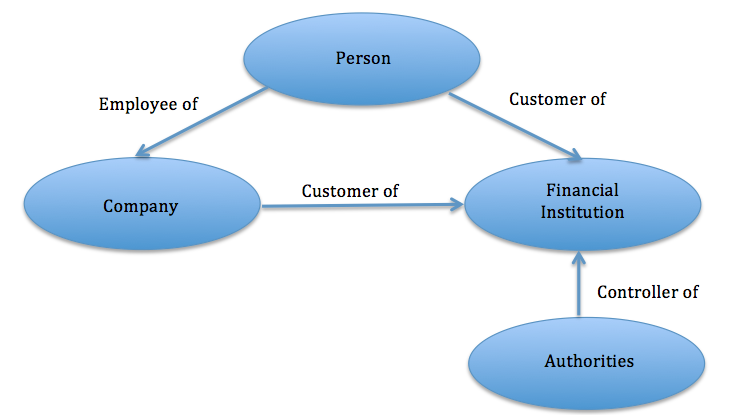
\includegraphics[width=\textwidth]{figures/Customers}
	\caption{Identities in the system}
	\label{fig:Customers}
\end{figure}
\subsection{Private Customers}
Private customers are the individual customers who access Nykredit services on their own. Usually there is a single person accessing the services of the bank. These customers are usually people who get a personal bank account with Nykredit.
\subsection{Corporate Customers}
Corporate customers are either companies who are customers of Nykredit or other financial institutions which provide Nykredit services to their own private customers. Usually there are many people who access Nykredit services on behalf of the corporate customer.
\section{Problem}
We consider the case of a person, who may either be a private customer of Nykredit, or an employee of a company who is corporate customer of Nykredit. In this case, the person may also be responsible for managing the accounts of his employer with Nykredit.
\\
\\Nykredit wants to setup an identity management system so that there is no need for the individual to disclose his personal identity to Nykredit to access the account on behalf of the company.
\\Nykredit, however, also have to comply with relevant legislation (KYC, AML, “Hvidvaskningsloven”),  e.g. in case the authorities (Tax, Police, etc.) find some suspicious transactions. Nykredit needs to provide the identity of the person responsible for these transactions.
This means that it is required that Nykredit, in case of a legal request, is able to identify the individual employee from the institution, who is accessing the account on the corporate customer’s behalf.
\\
\\So the main goal of the system is:
\begin{itemize}
	\item Nykredit should not learn identity of the individual person accessing the services on behalf of corporate customer.
	\item For complying with legislation Nykredit should be able to map real identity of the individual person with the transaction in case its required by the law.
\end{itemize}
The project will perform an initial analysis of a single business process from administrative data management, with respect to identifying the need to bind authenticated identities to actions at the different steps of the process; this analysis will be presented to stakeholders from the specific administrative domain. Based on the initial analysis of the selected business process, the project will develop a full identity model for the chosen business process with anonymisation and pseudonymisation of actors whenever possible. The feasibility of the proposed model will be evaluated through a prototype that implements the model using standard components from identity management infrastructures whenever possible.
\section{Summary}
Companies do not want to disclose the personal identity of their employees to Nykredit, but they still need the ability to access all services online. Managing all identities, while maintaining privacy, is not easy and provides different challenges. We have to design a system, which fulfill the entire privacy requirement and still enables Nykredit to provide its services to its customers and meet the regulatory requirements of the authorities without any problem.
                                  %Chapter 1
\chapter{State of the art Survey}

This chapter introduces some of the technologies currently available that deal with anonymity and privacy. Some of the technologies are already commercially available and being used in the industry, while others are still in research phase. We will give a brief introduction for all of them and a brief idea of how they can be used.

\section{Definitions and Common Terminology}
Below are the main terminologies and definitions used in this thesis:
\begin{itemize}
\item\textbf{Privacy :}
It is the ability of an individual to control the distribution of information about himself. An individual should be able to choose which information about him should remain secret and which information can be revealed.
\item\textbf{Anonymity :}
It refers to the ability of a user to not give any information about him at all to the system. It is the state of not being identifiable in the system. An anonymous system doesn't have any identity of the user.
\item\textbf{Pseudonym :}
It is a name given to the user in pseudonymous systems. This name is given to hide the real identity of the user from the system. The system only knows the user by his pseudonym.
\item\textbf{User :}
It is the end user of the system. It is the person who will go online and get the services. In our system, most of the time, we refer to user as the employee of the company, who is accessing the services of the bank.
\item\textbf{Bank :}
It is the financial institution which provides online financial services to the user. In our system, we refer to Nykredit as the bank.
\item\textbf{Third party :}
A third party or trusted third party is the entity which is neither the bank or the user in the system. A third party provides different services to banks or users and hence reduces the burden on them to setup all the infrastructure by themselves. In our system, Signicat is referred to as the third party.
\item\textbf{Service :}
It is something that is provided to the user online by a system. It may include the ability to login, check his account balance, upload pictures, share spreadhseets etc.
\item\textbf{Unlinkability :}
It is the privacy property where it is not possible to link 2 different entities to each other even though they are the same. 
e.g. not to be able to link 2 different sessions by the same user in the system.
\item\textbf{Revocation :}
It is the property where a user credential is revoked by the user or some other authority. After revocation, this credential cannot be used for anything.
\item\textbf{Partial Information Disclosure :}
It is the ability of a user to only disclose some partial information about himself to the system. e.g. a user might just want to disclose his last name to the system but not his full name.
\item\textbf{Legal Requirement :}
It is something that is required by law. e.g. it may be required by law that the bank logs all the customer data. Also sometimes in case of suspicious transactions the bank may be required legally to give the user identity to the relevant authorities.
\item\textbf{Conditional Anonymity Removal :}
It is the ability of the system to remove anonymity of the user if some conditions that were set before are met. This is mainly used for escrow purposes.
\item\textbf{Verifiable Encrytion :}
It is a type of encryption, in which encypted data can be verified i.e. someone who doesn't know the actual data can verify that the encrypted data is same as claimed by the person who encrypted it. e.g. if the person who is encrypting the data has to encrypt his key in it, it can be verified that he has encrypted his real key and not some garbage value.
\item\textbf{Zero Knowledge Proof :}
It is a type of proof where prover is able to convince the verifier about validity of a statement without giving any other information about the statement except that its valid. e.g. if a user have to prove that he has a private key to a particular public key, he can prove it without giving away any other information about his private key.
\section{Technologies}
After getting the requirements and based on our terminology we looked at the current technologies. We came out with a map as in figure \ref{fig:Technologies}. Basically we divided our type of technologies in 4 different types, depending on the functions:
\begin{enumerate}
	\item Secure Multi-Party Computing
	\item Escrow Technologies
	\item Identity Management Systems
	\item Zero Knowledge Technologies
\end{enumerate}
\begin{figure}[h]
	\centering
	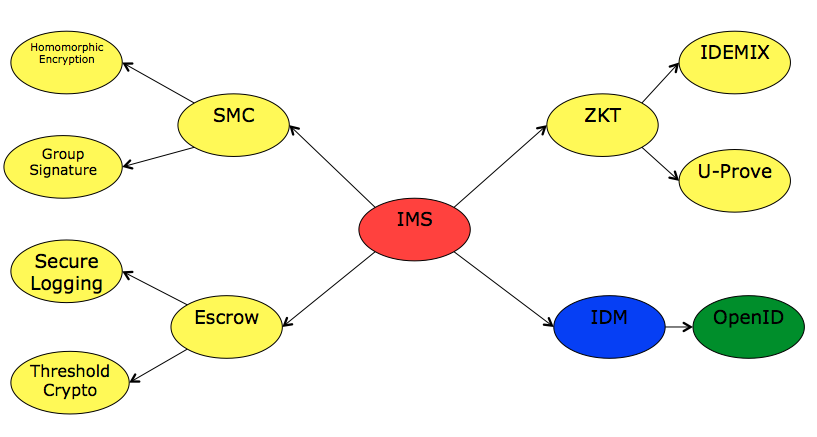
\includegraphics[width=\textwidth]{figures/Technologies}
	\caption{Technology Overview}
	\label{fig:Technologies}
\end{figure}
\section{Secure Multi-Party Computing}
These technologies are the ones which involve multiple parties to do computations. It is a subfield of cryptography which involves multiple parties getting an input and compute a joint function on them while keeping these inputs private. We basically looked at 2 technologies of interest here:
\subsection{Homomorphic Encryption}
Homomorphic encryption is a type of encryption where certain arithmetic operations can be performed on the ciphertext such that when the resultant ciphertext is decrypted, the decrypted text is same as the operations were performed on the plaintext. This is a new field of cryptography and is very useful where we need some parties to perform such operations without revealing the underlying data to those parties. Homomorphic encryption is also useful for chaining of different services without exposing data to any of those services.
\subsection{Group Signature}
A group signature is a scheme which allows a member of the group to sign the message on behalf of the group but anonymously. To outsiders the message has been signed by someone from the group but the exact identity of the person is now known. Also if the same member signs 2 different messages it is not possible to know if the message is signed by the same member. There is a notion of group manager in these scheme. Group manager is someone who manages the membership to the group. He can add/remove members from the group, find out who actually signed the message from the group. This scheme is useful where only thing that needs to be validated is that a certain person is part of the group, but his real identity is not required.
\section{Escrow Technologies}
Escrow technologies are the ones which are helpful in escrow purposes i.e. getting real data/identity later on in time from encrypted data if needed. We look at following 2 technologies.
\subsection{Secure Logging}
Secure logging is the process of saving the data in a secure manner. As saved data is really crucial and vulnerable to the attacks. We need to make sure that data is saved securely and its integrity is protected. This can be done in several ways. One way is to encrypt all the logs while storing them so that even if someone get hold of the logs, they can't use them without having access to the decryption key. Other way is to store logs at a third party after encrypting them. For escrow purposes, these logs can be decrypted later on with the decryption key.
\subsection{Threshold Cryptography}
Threshold cryptography is a field of public key cryptography where in order to decrypt an encrypted message, several parties must cooperate in the decryption. This message is encrypted using a public key and the corresponding private key is shared among different parties who will participate in the decryption process i.e. multiple parties hold the private key for a single public key. There is a term called threshold, and if there are \textit{n} parties who share the private key and at least \textit{t} parties which are required to decrypt the message such system is called (t,n) threshold cryptosystem. Threshold cryptosystem is useful in escrow purposes where a minimum number of parties can be defined to decrypt the ciphertext in order to get the plaintext.

\section{Identity Management Systems}
These are traditional identity management systems. For our purposes we look at OpenID system.
\subsection{OpenID}
OpenID is an open and decentralized protocol, which can be used to authenticate to different co-operating sites with the use of a third party service. It has notion of a \textit{relying party} and \textit{OpenID identity provider}.
\begin{itemize}
\item \textbf{OpenID Identity Provider} OpenID identity provider is the service, which actually provides authentication services. End user registers at OpenID identity provider to get his OpenID identity.
\item \textbf{Relying Party} Relying party is the website which user wants to authenticate to and which rely on the OpenID identity provider to provide authentication.
\end{itemize}
In addition to this an extension called \textit{OpenID attribute exchange} helps facilitate the transfer of user attributes from identity provider to the relying party
\begin{itemize}
\item User goes to the relying party service page
\item Service page presents different OpenID providers to login to the service
\item User chose the provider he has registered his openID with
\item Relying party redirects the user to the OpenID provider url so that user can authenticate
\item User can be authenticated by the method provided by OpenID provider
\item OpenID provider asks user the permission to share the attributes with the relying party
\item After user consent, user is redirected to the relying party website with user credentials
\item Relying party can verify the credentials and then login the user to the service
\end{itemize}
\section{Zero Knowledge Technologies}
These are the technologies which use the concept of zero knowledge i.e. proving knowledge about something without divulging the information. For our purpose we focus on mainly 2 technologies – IDEMIX and U-Prove, which are based on the concept of zero knowledge and verifiable encryption.. They both have a lot in common and have been studied a lot in industry. 
\subsection{IDEMIX}
U-Prove is a digital credential technology by IBM. it relies on anonymous credentials known as IDEMIX tokens. It is based on Camenisch-Lysyanskaya (CL) signature scheme which provides efficient zero-knowledge proofs. IDEMIX  have different entities in the system
\begin{itemize}
	\item \textbf{User} User is basically the entity, which is proving his identity in the system.
	\item \textbf{Verifier} Verifier is the entity, which verifies the identity of the prover.
	\item \textbf{Issuer} Issuer is the entity, which issues the credentials to the prover to prove his identity
	\item \textbf{Inspector} Inspector is the entity, which in case of discrepancy or legal requirement , can actually come and get the real identity of the prover.
\end{itemize}
\begin{figure}[h]
	\centering
	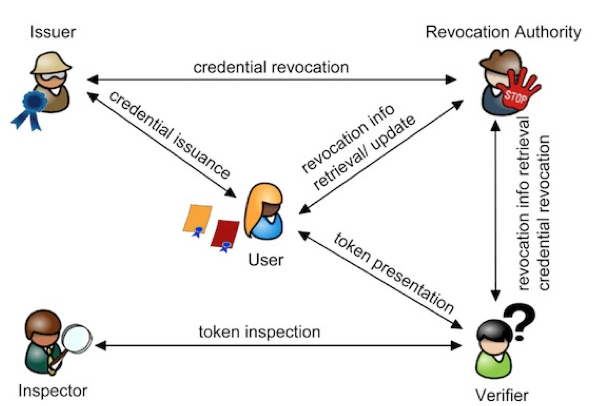
\includegraphics[width=\textwidth]{figures/Roles}
	\begin{minipage}{\textwidth}
		\footnotesize
		\emph{Source: https://github.com/p2abcengine/p2abcengine/wiki/Concepts-and-features}
	\end{minipage}
	\caption{IDEMIX Roles}
	\label{fig:Roles}
\end{figure}

For IDEMIX we need computing devices which work on behalf of each entity in the system.
\subsubsection{IDEMIX Credential}
An Idemix credential is CL Signature by issuer on user's private key and on attribute values. A user have independent public keys or pseudonyms for the same private key. These pseudonyms are IDEMIX tokens which are then used by the user to prove his identity to the different verifiers. IDEMIX has been studied a lot and many EU projects on anonymous credentials are based on it e.g. FutureID, ABC4Trust etc.
\begin{figure}[h]
	\centering
	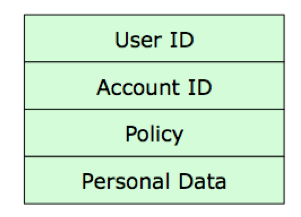
\includegraphics[width=170pt]{figures/Credential}
	\caption{IDEMIX Credential}
	\label{fig:Credential}
\end{figure}
\subsubsection{Issuance}
The first step is the credential issuance. It involves following steps:
\begin{itemize}
	\item User sends credential request to the issuer
	\item Issuer presents the issuance policy specifying
		\subitem Which attributes to present
		\subitem Which pseudonym/existing credentials to present
	\item Issuer also present a credential template specifying
		\subitem Which attributes of the new credentials will be generated at random
		\subitem Or carried over from existing credential or pseudonym
	\item User then present the issuance token satisfying the issuance policy
	\item Then multi-round cryptographic protocol ensues at end of which user get the IDEMIX credential
\end{itemize}
\subsubsection{Presentation}
Next step is to present the IDEMIX token for authentication to the verifier. It consists of following steps:
\begin{figure}[h]
	\centering
	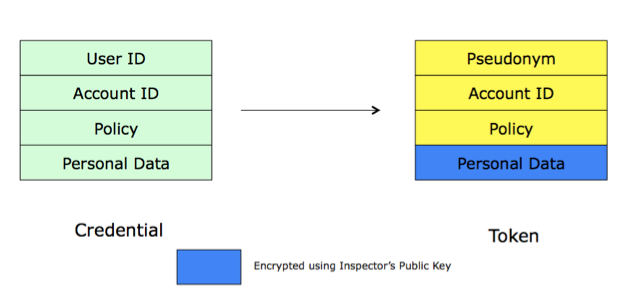
\includegraphics[width=\textwidth]{figures/Token}
	\caption{IDEMIX Presentation Token}
	\label{fig:Token}
\end{figure}
\begin{itemize}
	\item User get the presentation policy from the verifier which specifies
		\subitem Which credentials user must present
		\subitem What information user should reveal from these credential
	\item User generate a presentation token in accordance with the presentation policy revealing only the attributes necessary
	\item User present this presentation token to the verifier
	\item Verifier can then verify the attributes
\end{itemize}
\subsubsection{ID Escrow}
IDEMIX provides the ID escrow ability in case it is required. Following steps need to be followed for ID escrow purposes in IDEMIX:
\begin{itemize}
	\item The presentation policy can have following optional specifications for the purpose of ID Escrow
	\begin{itemize}
		\item Public keys of inspectors
		\item Attributes values to be encrypted using the keys	
		\item Inspection conditions under which these attributes can be revealed
	\end{itemize}
	\item User can prove that he has put these values in the presentation token with verifiable encryption to the verifier
	\item Once the token in presented, the inspection conditions are fixed and cannot be changed 
	\item In case of some discrepancy or legal requirement, an inspector can come and get the identity of the user from the token
\end{itemize}


\subsection{U-Prove}
U-Prove is a digital credential technology by Microsoft. It relies on anonymous credentials known as U-Prove tokens. It provides users a way to minimaly disclose their personal information while interacting with different online services. U-prove have different entities in the system
\begin{itemize}
	\item \textbf{Prover} Prover is basically the entity, which is proving his identity in the system.
	\item \textbf{Verifier} Verifier is the entity, which verifies the identity of the prover.
	\item \textbf{Issuer} Issuer is the entity, which issues the credentials to the prover to prove his identity
	\item \textbf{Auditor} Auditor is the entity, which in case of discrepancy or legal requirement , can actually come and get the real identity of the prover.
\end{itemize}
For U-Prove we need computing devices which work on behalf of each entity in the system.
\subsubsection{U-Prove Token}
U-Prove token is basically cryptographically protected information of any kind e.g. attributes. These are issued by issuer to the prover by issuance protocol. These tokens are then presented by prover to the verifier. Issuance and presentation of U-Prove tokens is unlinkable.
\subsubsection{Issuance}
The first step is the credential issuance. It involves following steps:
\begin{itemize}
	\item Prover invoke U-Prove issuance protocol
	\item Prover provides the attributes to be encoded
	\subitem Using \textit{Collaborative Issuance} property user can make sure that issuer doesn’t actually knows the attributes
	\item Then multi-round cryptographic protocol ensues at end of which user get the U-Prove token from the issuer
\end{itemize}
\subsubsection{Presentation}
Next step is to present the U-Prove token for authentication to the verifier. It consists of following steps:
\begin{itemize}
	\item Prover invoke the U-Prove presentation protocol
	\item User generate a presentation token in accordance with the presentation policy revealing only the attributes necessary
	\item User present this presentation token to the verifier
	\item Verifier can then verify the attributes
\end{itemize}
It must be noted that a revocation check can be added if needed before verifying the token.
\subsubsection{ID Escrow}
ID Escrow in U-Prove is actually an extension to existing U-Prove technology. It uses a type of ElGamal encryption which is verifiable.
\begin{itemize}
	\item  During the presentation protocol, prover proves that his ID is encrypted in the token by the use of verifiable encryption technology
	\item De-anonymization cannot be done by verifier or issuer
	\item A special entity called Auditor is responsible for de-anonymization in case of some discrepancy or legal requirement
	\item Threshold cryptography can be used in case of auditors and key can be split among multiple auditors.
\end{itemize}

All these different technologies provide different level of anonymization in the system. Some of them are easy to integrate in existing technology, while some are still not mature enough. For our purposes from now on we focus on mainly 2 technologies:
\begin{itemize}
	\item OpenID
	\item IDEMIX
\end{itemize}                                 %Chapter 2
\chapter{Application Scenario}
\section{Introduction}
Here we will discuss the application scenario of the technologies discussed in chapter two. Most of it will be based on the models we described in the requirement document and also banking document.
In this chapter we will try to describe our understanding of the current banking system. We will give different types of data that exist in the current system and the different operations that it is necessary to support in the system.
\section{Components}
We have identified following four components that the bank needs to maintain in its relationship with its customers. Together, these four components define a customer engagement:
\begin{itemize}
\item ID
This is the main identity of the user. The user is identified in the system using this ID. This ID can be anything from a pseudonym, as in the numbered Swiss bank accounts, to the verified real world identity (CPR number) of the customer used in Danish banks. 
\end{itemize}
\begin{itemize}
\item Basic Data
Related to the ID is the basic data of the user. This data is the data that is required by the bank to identify the customer in real life and maintain its relationship with the customer. Basic data can consist of the following:
\begin{itemize}
\item Name
\item Address
\item Email ID
\item Phone Nr.
\item CPR nr.
\item Marital Status
\item Gender
\item Date of Birth
This is the most basic form of data which describes a single customer and which rarely changes. It can include some other data that might be crucial for the bank.
\end{itemize}
\end{itemize}
\begin{itemize} 
\item Account 
Next component in the chain is the account of user with the bank. The account component holds all the static information regarding the account. Examples of such information are:
\begin{itemize}
\item Account Nr.
\item Account Type
\item Owner ID
\item Interest rate
\item Balance
\item Account opening date
\item Overdraw limit
As before it can include some other data that might be needed to operate the account or that might be crucial for the bank.
\end{itemize}
\end{itemize} 
\begin{itemize}
\item Transaction History
The transaction history includes all the dynamic data that the bank has on a particular account. Typical transactions are:
\begin{itemize}
\item Deposits
\item Withdrawals
\item Accruing Interests
\end{itemize}
\end{itemize} 
\begin{itemize}
\item Authorization and Access Control
In the following, we identify the most basic operations needed to maintain the information above and the customer/bank relationship. This includes the operations that are permitted on the accounts. We represent it in our system as an API, which takes an input, and perform the desired operation. Some examples can be:
\begin{itemize}
\item Deposit (ID, Account Nr., Amount)
This is the most basic operation. This will take user ID, Account Nr. and deposit the amount in the account.
\item Withdraw (ID, Account Nr., Amount)
This will take user ID, Account Nr. and withdraw the amount from the account.
\item Transfer (ID, Account Nr. 1 Account, Nr. 2, Amount)
This will take user ID of the person initiating the transfer, Account Nr. 1, Account Nr. 2 and transfer the amount from Account Nr. 1 to Account Nr. 2.
\item Close Account (ID, Account Nr.)
This will take user ID, Account Nr. and close the account.
\item Open Account (ID)
This will take user ID and open an account for the given user ID.
\item Actions (ID, Account Nr., ID1, Action1, ID2, Action2,…., IDn, Actionn)
This will take user ID, Account Nr. and other IDs and Actions that those IDs are allowed to do on the account and then will create a policy for those IDs in the database.
For all above operations we assume that ID is authorized to perform such operations.
\end{itemize}
\end{itemize}                                  %Chapter 3
\chapter{Proposed System}
\section{Introduction}
This chapter will present our proposed system as the solution. We will define our system and show how it solves the problem of privacy of the users.
                                 %Chapter 4
\chapter{Simple Prototype}
\section{Introduction}
This chapter will deal with our Identity management based solution. Mainly we will talk about OpenID solution here. And how this solution will apply to the application scenario discussed in chapter 3.                                 %Chapter 5
\chapter{IDEMIX Based Solution}
In this chapter we will provide a solution using IDEMIX based IMS. We will give more details about how this system can be implemented, and how will it behave for the end users.
\section{IDEMIX IMS}
As in previous case we can replace IMS with IDEMIX based IMS in our pseudonymous system. This system will take user credentials and then send an IDEMIX token to the bank. This IDEMIX token contains pseudonym as well as account ID and policy for the user. This IMS can be controlled by a separate identity inside the bank or by a 3rd party.
\begin{figure}[h]
	\centering
	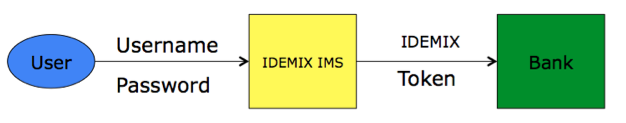
\includegraphics[width=\textwidth]{figures/IDEMIX}
	\caption{Pseudonym System with IDEMIX IMS}
	\label{fig:IDEMIX}
\end{figure}
\section{System Setup}
The system can be setup in 2 ways:
\begin{itemize}
	\item IMS controlled by a separate department at bank.\\
	In this case the bank separate the authentication and service part in 2 different departments internally. Authentication is controlled by IMS which holds the IDEMIX credentials for the user. Service department only gets the IDEMIX token from the authentication department.
	\item IMS controlled by a third party\\
	In this case the bank operates the service part while the authentication part is operated by a trusted third party.
\end{itemize}
In both cases, bank and IMS have to collaborate. Bank have to trust the IMS system that IDEMIX token sent by the the IMS system is correct.
\subsection{Changes on the Bank Side}
In this system, bank needs to behave as an IDEMIX issuer and verifier. It will issue IDEMIX credentials for the users and also will verify the tokens sent by the IMS system. 
\subsection{Information Stored at IMS}
IMS system will behave like user in the IDEMIX system. IMS needs following user information to be stored
\begin{itemize}
	\item User IDEMIX credential
\end{itemize}
Account ID and policy can be stored in encrypted form in the credential itself. This IDEMIX credential for a particular user can be setup in the beginning and then can be used later to create authentication tokens.
\subsection{Changes needed on the User Side}
On user side no changes are needed. User access the system like before. User doesn't need to install any special software or hardware on his side to access the bank services. 
\section{User Creation}
Following are the steps for creation of a new user account in OpenID based system
\begin{itemize}
	\item User goes to bank to open a new account.
	\item User provides his details.
	\item Bank creates user policy and send this information to the IMS system along with other user information as an IDEMIX credential.
	\item IMS system verifies the IDEMIX credential for the user and provides user with credentials to access his account.
	\item User then can login to his account using the credentials.
	\item In case of corporate users, if user is the administrator then he can add more users using a web interface at the bank directly and decide account policies for those users.
\end{itemize}
\section{User Authentication}
Authentication steps are as following in IDEMIX based system
\begin{itemize}
	\item User goes to login page
	\item User provides his username and password
	\item This is sent to IDEMIX IMS which then gets the saved user credential and creates a presentation token with a pseudonym for the bank
	\begin{itemize}
		\item Also for escrow purposes the real user identity is also encrypted in the token with the public keys of authorities
	\end{itemize}
	\item Bank receives this presentation token and gets the following information
	\begin{itemize}
		\item Pseudonym
		\item Account ID
		\item Policy
	\end{itemize}
	\item Bank adds this information in a temporary policy database
	\item Bank saves the token for future escrow purposes
	\item User can then access services from the bank using the pseudonym
	\item All user transactions are logged with the pseudonym
\end{itemize}
\section{ID Escrow}
Following are the steps for ID escrow in IDEMIX based system
\begin{itemize}
	\item Authorities come to the bank for transaction data and IDEMIX token.
	\item After verifying, bank gives the transaction data and corresponding IDEMIX token to the authorities.
	\item Authorities then using their key get the real identity of the user from the IDEMIX token.
\end{itemize}
\section{Analysis}
With the use of IDEMIX IMS we add a pseudonymous layer in the system. This provides us the necessary privacy. In order to do so, IDEMIX IMS just need to store the IDEMIX credential of the user. 

The provider doesn’t need to store any mapping database on his side. It is easier for bank to implement, as bank really doesn’t have to trust the IDEMIX IMS to store sensitive data.

In case there is a discrepancy, the authorities need to go only to the bank to get the transaction data as well as the mapping data from the IDEMIX tokens.
\section {IDEMIX implementation in the Real World}
Now we will try to fit this implementation in our system, which includes Nykredit as the Bank, Signicat as the 3rd party, DTU as corporate customer and other government institutions as authorities.
\subsection{Addition of the New User}
Addition of the new user can happen as following:
\begin{enumerate}
	\item DTU registers the new user with the Nykredit giving them the user details and policies that should apply to the particular user regarding the account. 
	\begin{enumerate}
		\item Nykredit registers this new user with his User ID with the IMS system
	\end{enumerate}
	\item Nykredit issue an IDEMIX policy credential for the given user to DTU. This credential contains the policy information and account information for the user.
	\item DTU then use this policy credential to register the new user with Signicat. 
	\begin{enumerate}
		\item Signicat inquire about the user data with the authorities
		\item Authorities verify the user data to Signicat
	\end{enumerate}
	\item After that Signicat issue final IDEMIX credential for the IMS system. This credential is then used to create pseudonym IDEMIX tokens for the user. 
\end{enumerate}
\begin{figure}[h]
	\centering
	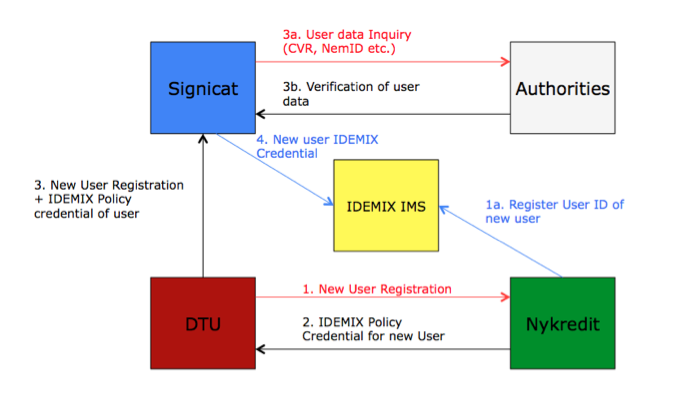
\includegraphics[width=\textwidth]{figures/IDEMIX-Real}
	\caption{IDEMIX Registration for a new user}
	\label{fig:IDEMIX-Real}
\end{figure}
\begin{figure}[h]
	\centering
	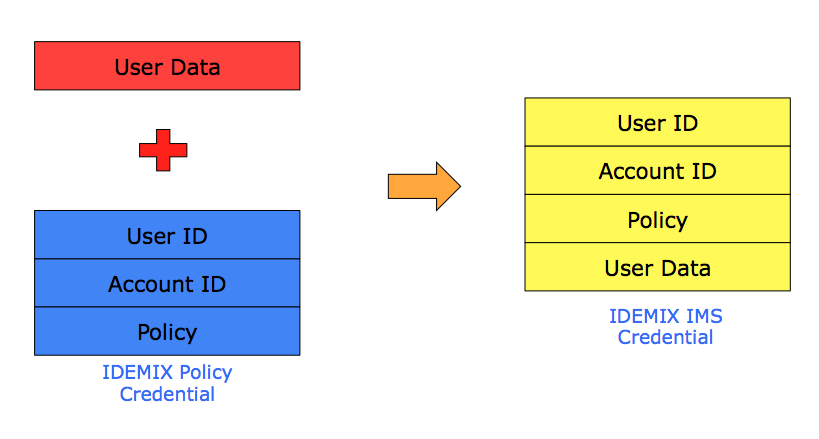
\includegraphics[width=\textwidth]{figures/Final}
	\caption{Final IDEMIX Credential from Policy Credential}
	\label{fig:Final}
\end{figure}
\FloatBarrier
\subsection{Addition of a New Customer}
Addition of the new customer is almost same as addition of new user:
\begin{enumerate}
	\item An administrator goes to Nykredit to open a bank account on behalf of DTU 
	\begin{enumerate}
		\item Nykredit registers DTU as new customer in their internal system.
		\item Nykredit registers the DTU administrator with his User ID with the IMS system
	\end{enumerate}
	\item Nykredit issue an IDEMIX policy credential for the  DTU administrator to himself. This credential contains the policy information and account information for the administrator.
	\item Administrator then use this policy credential to register himslef as owner of the new DTU account with Signicat. 
	\begin{enumerate}
		\item Signicat inquires about the data given in the credential with the authorities
		\item Authorities verify the data to Signicat
	\end{enumerate}
	\item After that Signicat issue final IDEMIX credential for the IMS system. This credential is then used to create pseudonym IDEMIX tokens for the administrator. 
\end{enumerate}
\subsection{Technical Requirements}
In this system DTU as a client does not need to change anything on their side to be a customer at Nykredit. All the system for DTU is web based where they can just add/remove users and also DTU users login to the system using the browser.

Nykredit have to implement IDEMIX issuer service on their side to issue IDEMIX Policy credential. This is done so that Nykredit doesn’t have to store the sensitive data at the 3rd party. Use of this credential ensures that this data remains safe. Nykredit also have to implement IDEMIX verifier service to verify the user identity.

Signicat have to implement IDEMIX issuer service also to issue final IDEMIX credentials.

IMS have to implement IDEMIX user service to create the IDEMIX tokens for the user while user is logging in.
\section{High Level Protocol Description}
In this section, we will give protocol description of the IDEMIX based system. This is a high level description of the protocol and full details can be found in \cite{camenisch2001efficient}.

We assume that all the systems are secured and all the communication within them is encrypted. Let $Cred_{I,U}(data1,data2,...)$ be an IDEMIX credential issued by issuer I to user U. We define DTU employee as entity D, Nykredit as entity N, IMS as entity I, Signicat as entity S and authorities as entity A. Also the notation
\begin{center}
$A->B : \{m\}$
\end{center}
means that a message $m$ is sent from $A$ to $B$ in encrypted form such that only A and B can read it.
We take 3 cases:

\begin{enumerate}
\item User Registration
\item User Authentication
\item User transaction
\end{enumerate}
	
\subsection{User Registration}
The first part of protocol is the user registration. It involves all the parties in the system. The details of the protocol are as below:
\begin{enumerate} 
\item 	Let  $username$ be the login name of the new user that DTU wants to give access to their account, $account\_id$ be the account number of DTU account with Nykredit and $policy_D$ be the policy defined by the DTU for the user on their account. DTU sends this information to the bank for the user registration.

\begin{center}
	$D -> N : \{username,account\_id,policy_D\}$
\end{center}
\begin{enumerate}
	\item Bank registers this new user with the IMS system with the given username and receives the password for user to login to the system.
	\begin{center}
		$N -> I : \{username\}$
		
		$I -> N : \{username,password\}$
		
	\end{center}	
\end{enumerate}
\item DTU sends this password as well as an IDEMIX credential for the given username back to DTU.
	\begin{center}
		$N -> D : \{username,password,Cred_N(username,account\_id,policy_N)\}$
	\end{center}	
Where $policy_N$ is the policy created by Nykredit for the user for the given account. It is a mix of the policy given ty the DTU and also some internal Bank policies. $Cred_N(username,account\_id,policy_N)$ is the IDEMIX credential issued by Nykredit for the user with given username.
\item DTU sends the user data and credential given by Nykredit to Signicat. This user data may contain \textit{real name,CPR nr,address,contact information} etc. for the user. 
\begin{center}
	$D -> S : \{username,userdata,Cred_N(username,account\_id,policy_N)\}$
\end{center}
\item Signicat verifies the user data with the authorities and then issue its own credential $Cred_S(userdata,Cred_N(account\_id,policy_N))$ for the user. This credential contains data from the Nykredit credential $Cred_N(account\_id,policy_N))$ also. This makes sure that Signicat is able to issue the credential over parameters given by Nykredit credential but have no access to the data inside.

Signicat sends this data to IMS system and user is registered with his credential in the IMS system.
\begin{center}
	$S -> I : \{username,Cred_S(userdata,Cred_N(account\_id,policy_N))\}$
\end{center}
User can now login to the system with IMS using his username and password.
\end{enumerate}

\subsection{User Authentication}


This chapter described the IMS system setup using the IDEMIX system. We described how the system would be setup and how it would affect all the parties involved.


                                 %Chapter 6
\chapter{IDEMIX Based Solution}
\section{Introduction}
In this chapter we will provide a solution using IDEMIX based IMS. We will give more details about how this system can be implemented, and how will it behave for the end users.
\section{IDEMIX IMS}
As in previous case we can replace IMS with IDEMIX based IMS in our pseudonymous system. This system will take user credentials and then send an IDEMIX token to the bank. This IDEMIX token contains pseudonym as well as account ID and policy for the user. This IMS can be controlled by a separate identity inside the bank or by a 3rd party.
\begin{figure}[h]
	\centering
	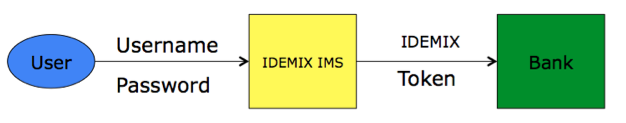
\includegraphics[width=\textwidth]{figures/IDEMIX}
	\caption{Pseudonym System with IDEMIX IMS}
	\label{fig:IDEMIX}
\end{figure}
\section{System Setup}
The system can be setup in 2 ways:
\begin{itemize}
	\item IMS controlled by a separate department at bank.\\
	In this case the bank separate the authentication and service part in 2 different departments internally. Authentication is controlled by IMS which holds the IDEMIX credentials for the user. Service department only gets the IDEMIX token from the authentication department.
	\item IMS controlled by a third party\\
	In this case the bank operates the service part while the authentication part is operated by a trusted third party.
\end{itemize}
In both cases, bank and IMS have to collaborate. Bank have to trust the IMS system that IDEMIX token sent by the the IMS system is correct.
\subsection{Changes on the Bank Side}
In this system, bank needs to behave as an IDEMIX issuer and verifier. It will issue IDEMIX credentials for the users and also will verify the tokens sent by the IMS system. 
\subsection{Information Stored at IMS}
IMS system will behave like user in the IDEMIX system. IMS needs following user information to be stored
\begin{itemize}
	\item User IDEMIX credential
\end{itemize}
Account ID and policy can be stored in encrypted form in the credential itself. This IDEMIX credential for a particular user can be setup in the beginning and then can be used later to create authentication tokens.
\subsection{Changes needed on the User Side}
On user side no changes are needed. User access the system like before. User doesn't need to install any special software or hardware on his side to access the bank services. 
\section{User Creation}
Following are the steps for creation of a new user account in OpenID based system
\begin{itemize}
	\item User goes to bank to open a new account.
	\item User provides his details.
	\item Bank creates user policy and send this information to the IMS system along with other user information as an IDEMIX credential.
	\item IMS system verifies the IDEMIX credential for the user and provides user with credentials to access his account.
	\item User then can login to his account using the credentials.
	\item In case of corporate users, if user is the administrator then he can add more users using a web interface at the bank directly and decide account policies for those users.
\end{itemize}
\section{User Authentication}
Authentication steps are as following in IDEMIX based system
\begin{itemize}
	\item User goes to login page
	\item User provides his username and password
	\item This is sent to IDEMIX IMS which then gets the saved user credential and creates a presentation token with a pseudonym for the bank
	\item Also for escrow purposes the real user identity is also encrypted in the token with the public keys of authorities
	\item Bank receives this presentation token and gets the following information
	\begin{itemize}
		\item Pseudonym
		\item Account ID
		\item Policy
	\end{itemize}
	\item Bank adds this information in a temporary policy database
	\item Bank saves the token for future escrow purposes
	\item User can then access services from the bank using the pseudonym
	\item All user transactions are logged with the pseudonym
\end{itemize}
\section{ID Escrow}
Following are the steps for ID escrow in IDEMIX based system
\begin{itemize}
	\item Authorities come to the bank for transaction data and IDEMIX token.
	\item After verifying, bank gives the transaction data and corresponding IDEMIX token to the authorities.
	\item Authorities then using their key get the real identity of the user from the IDEMIX token.
\end{itemize}
\section{Summary}
This chapter described the IMS system setup using the IDEMIX system. We described how the system will be setup and how it will affect all the parties involved. We will analyze this system later in chapter 8.

                                 %Chapter 7
\chapter{Conclusion and Future work}
This chapter will conclude the thesis and will provide directions for the future work that can be carried out in the field.
\section{Conclusion}
To conclude, we can say that technology is changing at an alarming rate. Service providers want to catch up with the technology advances and address the privacy issues currently prevalent. But its not easy as they are not yet ready to give up on the legacy systems. Also its difficult to make radical changes in already running systems. 

Service providers still rely on the user data they have stored to provide their services and its difficult to remove that reliability at once. These changes cannot be made overnight but it will take some time for industry to understand the value in changing their business processes to not to rely on user data. 
\section{Future Work}
Providing anonymity in business processes is an interesting field of research both for industry and academics. This section provides some insights on how the systems presented in the thesis may affect future research in the area and how it can be used in some alternate ways by industry to provide the services.
\subsection{Reidentification possibilities}
In our sytems we have removed the identification from the transactions. As mentioned in \cite{de2015unique} the researcher were able to reidentify individuals based on the credit card transactions from past 3 months. Even though all those transactions were completely anonymized. It would be interesting to put our system in the place and use the same methodology to see if individuals can be reidentified.
\subsection{Providing services using the third party}
One more aspect, as we see from our point is that our system has removed identity from the service part of the businesses. As most of the businesses are moving towards outsourcing their IT divisions for cost cutting purposes our system provides them a unique opportunity to do so. As there is no identity involved in the service system, the whole service side can be outsourced without the risk of giving away confidential data to the third parties.

Finally with this chapter concluded the thesis and provided some insights on future work that can be done in the field.

                                 %Chapter 8
\chapter{Conclusion and Future work}
\section{Introduction}


                                 %Chapter 9
\chapter{Conclusion and Future work}
\section{Introduction}
Final chapter will conclude the thesis and will give some directions to the future work that can be done in the field.
                                %Chapter 10
\appendix
\chapter{Appendix A}

This appendix is full of stuff ...                                %Appendix 1
%-----------
% Backmatter
%-----------
\backmatter
\chaptermark{Bibliography}
\renewcommand{\sectionmark}[1]{\markright{#1}}
\sectionmark{Bibliography}
\addcontentsline{toc}{chapter}{Bibliography}        %Force addition of Bibliography to TOC
%\bibliographystyle{alpha}                           %Use alpha codes for references
\bibliographystyle{ieeetr}                       %Use IEEE codes for references
\nocite{*}
\bibliography{References}                           %Bibliography file called

\end{document}
% % % EOF % % %